%  Robotics Text  by Jacob Rosen and Blake Hannaford
% (c) 2007  Jacob Rosen and Blake Hannaford
%

\chapter{Trajectory Generation}\label{ChapterTrajectoryGeneration}

\section{Problem Statement and Learning Objectives}
% Problem Statement and Learning Objectives for Chapter 07

\paragraph{Problem Statement}
  
If a manipulator is asked to move from one pose to another, it must do so smoothly and with speed and acceleration which is under the control of the programmer.  
This chapter describes techniques for generating smooth trajectories between two positions of the robot manipulator.  Mathematically this problem can be thought of as that of finding a function of time which meets specified boundary conditions and other constraints.  

\paragraph{Learning Objectives} After completing this chapter, the student will be able to
\begin{itemize}
  \item Design or program linear trajectories with parabolic start and stop periods.
  \item Design or program trajectories based on cubic polynomials.
  \item Design or program trajectories which are constrained to move through via points.
  \item Design trajectories for the joints of a robot arm which result in straight trajectories in Cartesian space.
\end{itemize}


\section{Trajectory Generation}

\begin{figure}\centering
\includegraphics[width=12.5cm]{figs07/00520.eps}
\caption{Most control analysis and design focuses on step inputs.}\label{stepinputdesign}
\end{figure}



Much of control theory focuses on the response of the system to a step input (Figure \ref{stepinputdesign}).  There are good historical and contemporary reasons for this focus, but it is often inappropriate for motion control systems including robotics.  Although no physical system can accurately follow the instantaneous position change of a step input, when viewed through the lens of control systems theory, the object is to design a controller which achieves desireable characteristics in the error.  For example, the designer may adjust controller parameters to get fast response with overshoot or slow response without overshoot.

\begin{figure}\centering
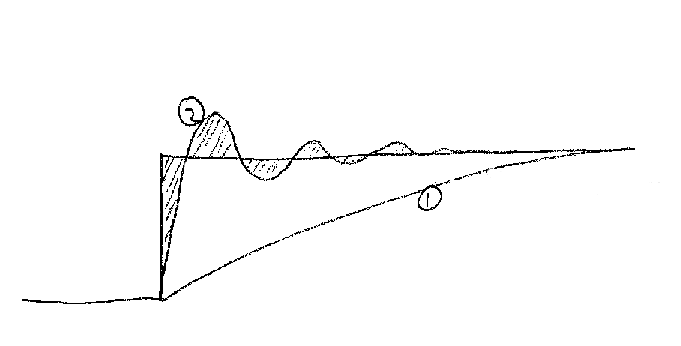
\includegraphics[width=10.5cm]{figs07/00521.eps}
\caption{There is usually a significant error between the output of a well designed control system and a step input.}\label{stepresponseerror}
\end{figure}


In both cases however, there is a large error between input and output (Figure \ref{stepresponseerror}).   In this chapter we will avoid the problem of tracking a step input by changing to a smoother input.  Such an input will demand lower velocities and accelerations and thus generate smaller tracking errors.  Overshoot can be particularly bad when a robot operates in a crowded environment.


\section{Joint Space Trajectory Generation}
Suppose one joint of a robot arm needs to go from
\[
\theta_A \to \theta_B
\]
in an amount of time $t_f$.
The problem of trajectory generation boils down to specifying a time function $\theta(t)$ such that
\[
\theta(0) = \theta_A \quad \mathrm{and} \quad \theta(t_f) = \theta_B
\]
In addition, we will initially assume the manipulator should be at rest before and after the move giving
\[
\dot{\theta}(0) =  \dot{\theta}(t_f) = 0
\]

The shortest distance between two points is a straight line.  This naive approach to generating a trajectory gives us
\[
\theta(t) = \theta_A + t \times \frac{\theta_B-\theta_A}{t_f}
\]

However, because we have assumed the velocity at $t=0^- $ and $t_f^+ = 0$, our acceleration must be infinite at the start and end of the trajectory.  No robot can accelerate that fast and so we will have significant tracking error.   Before we start looking at some candidate functions then, we should think about what we want in the function $f(t)$.    We will consider a trajectory a ``good" one if it satisifies two criteria:  ``Smoothness" and ``Attainability".

We will consider the function smooth if $\theta(t)$ and $\dot{\theta}(t)$ are continuous.

We will consider the function attainable if $|\ddot{\theta}(t)| \leq \ddot{\theta}_{MAX}$.

There are   many possible functions which could meet these criteria.  We will consider two in depth,

\begin{enumerate}
\item A polynomial
\item A linear function with parabolic start and end regions to limit maximum acceleration.
\end{enumerate}


\subsection{3rd Order Polynomial}\label{3rdPoly}

\begin{figure}[h]\centering
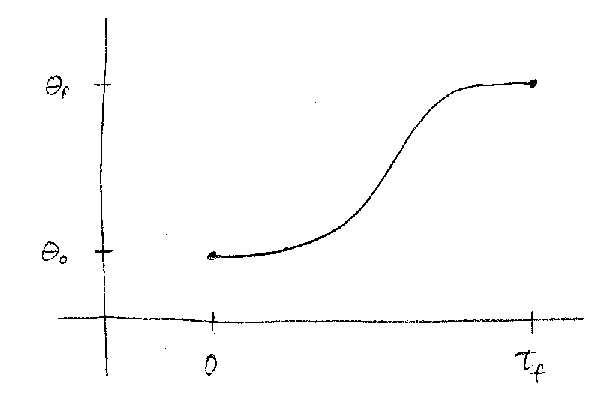
\includegraphics[width=10cm]{figs07/00510.eps}
\caption{With the right coefficients, a third order polynomial can make a smooth trajectory between two values in a finite time.}\label{thirdorderpolyfigure}
\end{figure}


A simple trajectory to start with is the 3rd order polynomial (Figure \ref{thirdorderpolyfigure}).  We need a function of the form
\[
\theta(t) = a_0 + a_1t + a_2t^2 + a_3t^3
\]
with the following boundary conditions
\[
\theta(0) = \theta_A		\qquad   \dot{\theta}(0) = 0
\]
\[
\theta(t_f) = \theta_B	\qquad   \dot{\theta}(t_f) = 0
\]
There are four unknowns ($a_0 \to a_3$) and the four equations above.
By differentiating and applying the boundary conditions we can obtain
\[
a_0 = \theta_A		\qquad a_1 = 0
\]
\[
 a_2 = \frac{3(\theta_B-\theta_A)}{t_f^2}	\qquad   a_3 = \frac{-2(\theta_B-\theta_A)}{t_f^3}
\]

Note that the derivatives are easy to compute analytically:

\[
\dot{\theta}(t) = 2a_2t + 3a_3t^2	\qquad \ddot{\theta}(t) = 2a_2 + 6a_3t
\]

The resulting trajectory and its derivatives looks like Figure \ref{pvathirdorder}.

\begin{figure}\centering
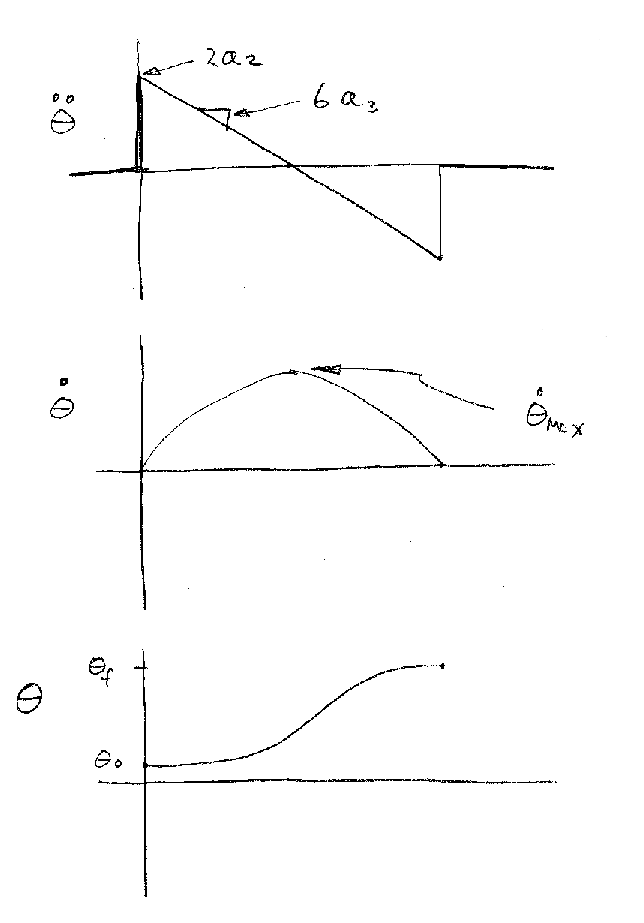
\includegraphics[width=9.5cm]{figs07/00511.eps}
\caption{Position ($\theta$), velocity ($\dot{\theta}$), and acceleration($\ddot{\theta}$)}\label{pvathirdorder}
\end{figure}


We can also easily get:
\[
\ddot{\theta}_{MAX} = \ddot{\theta}(0) = 2a_2 = \frac{6(\theta_B-\theta_A)}{t_f^2}
\]
\[
\dot{\theta}_{MAX} = \dot{\theta}(t_f/2) = \frac{3}{2}\frac{(\theta_B-\theta_A)}{t_f}
\]

This function meets our requirements for smoothness and attainability if
\[
\ddot{\theta}_{MAX} \geq 2a_2
\]








\begin{ExampleSmall}
Design a 3rd order polynomial trajectory with $\theta_A = 40^\circ$, $\theta_B=120^\circ$, $t_f = 2.4$sec.   Also derive  the velocity and acceleration of the trajectory:

ANS:

\[
a_0 = 40^\circ
\]
\[
a_2 = \frac{240^\circ}{2.4^2} = 41.67
\]
\[
a_3 = \frac{-2\times80^\circ}{13.824} = -11.57
\]
\[
\theta(t) = (40 + 41.67t^2 - 11.57 t^3)^\circ
\]
by differentiation:
\[
\dot{\theta}(t) = 83.34t - 34.71t^2
\]
\[
\ddot{\theta}(t) = 83.34 - 69.42t
\]
\end{ExampleSmall}







\subsection{Linear with Parabolic Blends}
To understand this trajectory, it is easiest to look first at the velocity curve of Figure \ref{linearparabolic}.


\begin{figure}\centering
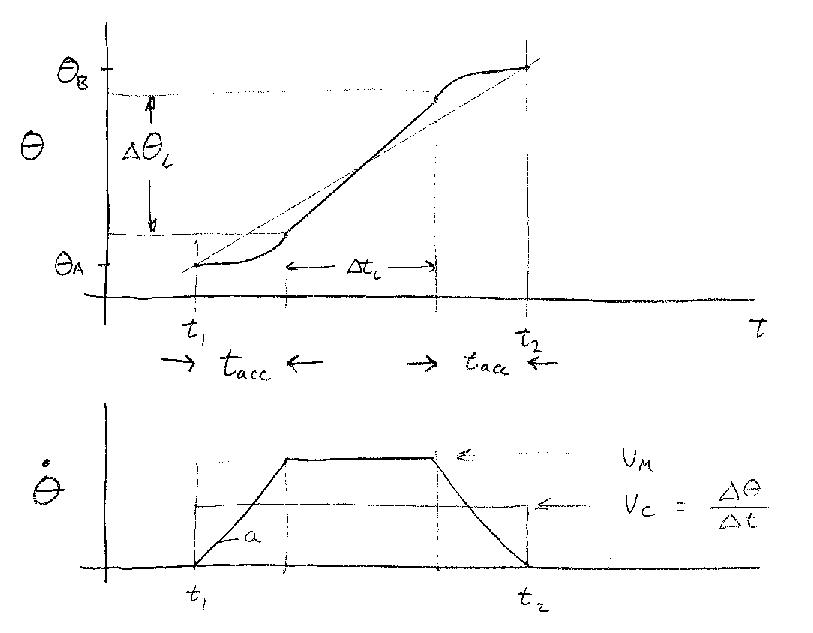
\includegraphics[width=13cm]{figs07/00512.eps}
\caption{A smooth three-segment trajectory can be formed by a parabola, a straight line, and another parabola.  This trajectory is defined by the time interval and the limits on velocity and acceleration. }\label{linearparabolic}
\end{figure}



Using this trajectory type, the velocity increases linearly for a time interval $t_{acc}$, then continues at a constant velocity, $V_M$, and then decreases linearly to zero for $t_{acc}$ seconds prior to the end of the trajectory.  The key constraint is that the area under the velocity curve must be equal to the displacement, $\theta_B-\theta_A = \Delta\theta$.  The area of the velocity curve is $V_M(t_2-t_1-t_{acc})$.  Thus:
\[
V_M(t_2-t_1-t_{acc}) = \Delta\theta
\]
\[
V_M = \frac{\Delta\theta}{t_2-t_1-t_{acc}}
\]
We can further obtain the acceleration of the velocity ramp, $a$
\[
a = \frac{V_M}{t_{acc}} = \frac{\Delta\theta}{t_{acc}(t_2-t_1-t_{acc})}
\]

Implementation of this trajectory in software is a bit more complex than the polynomial.  We must divide the trajectory time into three phases:  acceleration, cruising, and deacceleration.


\begin{ExampleSmall}
Write pseudo code to generate a linear trajectory with parabolic blends.   Divide your code into two functions, one which plans the trajectory and returns the constants $V_M, a$ etc. and a second one which is called every 0.001 seconds and computes $\theta(t)$.  Make sure that acceleration is not greater than a predefined {\tt A\_MAX}.

ANS:

\begin{verbatim}
\\ generate constants
lin_parab_init(float delta_theta, float delta_t)
 {
 t_acc = 0.25 * delta_t; // arbitrary, other ways could be better
 VM = delta_theta/(delta_t - t_acc);
 a = VM / tacc;
 if(abs(a) > A_MAX) { error("Acceleration too high"); }
 }

\\run time call
lin_parab_run(float t, float t_0, float theta_A, float delta_t,
                                 float t_acc, float a, float VM)
 {
 dt = t-t_0;
 if(dt < t_acc) { // acceleration phase
   return(0.5 * a * (t-t_0)^2 + theta_A);
   }
 else if (dt > t_acc && dt < delta_t-t_acc) { // cruise
   return(0.5 * t_acc*VM + VM*(t-t_0-t_acc) + theta_A);
   }
 else if (dt > delta_t - t_acc) {  // decceleration
   return((theta_A+delta_theta)- 0.5*a*(t-delta_t)^2);
   if(t == delta_t)  stop;
   }
 }

\end{verbatim}

\end{ExampleSmall}



\subsection{Via Points}

We may need to specify an intermediate point between a start and a goal.  For example, in Figure \ref{cornerviapoint}, starting at the point A, we must go to the point V before B in order to avoid the obstacle.



\begin{figure}\centering
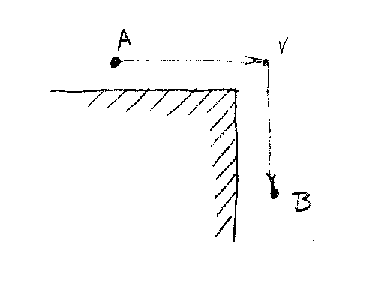
\includegraphics[width= 4.5cm]{figs07/00513.eps}
\caption{An intermediate (via) point must be established to avoid the corner-shaped obstacle.}\label{cornerviapoint}
\end{figure}



If we translate the three points, $A, V, B$,  to joint configuration, and we consider just one joint, we need a trajectory something like one of the two trajectories shown in Figure \ref{viatrajectoryoptions}.  In the first option (left) the joint value corresponding to the Via point $\theta_V$ is outside the range between $\theta_A$ and $\theta_B$.  In the second, (right) $\theta_A < \theta_V < \theta_B$.

\begin{figure}\centering
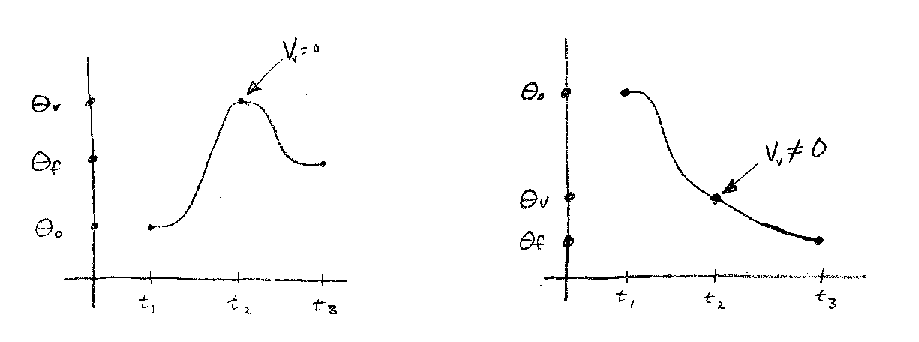
\includegraphics[width=14.5cm]{figs07/00514.eps}\caption{Two possible smooth trajectories combining trajectory $AV$ and trajectory $VB$. (need to correct subscripts in graphics.}\label{viatrajectoryoptions}
\end{figure}




In the example at left, we need to go through zero velocity at point V but in the case at right it would break up the motion to require zero velocity at the via point.   We should specify some non zero velocity at the via point for smoother motion.   We could allow the user to specify this velocity.  Alternatively, to automatically generate it, we can use some heurisitics such as
\begin{enumerate}
  \item if the difference in $\theta$ changes sign, $V_V = 0$.
  \item if not, average the slopes:
\[
  V_V = 1/2 \left ( \frac{\Delta\theta_1}{\Delta_{t1}} + \frac{\Delta\theta_2}{\Delta_{t2}} \right )
\]
\end{enumerate}

Once we have derived a value for the velocity in the via point, $V_V$, we can compute the new trajectory as follows:

First, redo the derivation of Section \ref{3rdPoly} but alter the boundary conditions:

\[
\dot{\theta}_1{(t_2)} = \dot{\theta}_2(t_2)
\]
Where the left hand side is the final velocity of the first sub-trajectory, and the right hand side is the initial velocity of the second sub-trajectory.

Alternatively, we can require that the acceleration, $\ddot{\theta}(t)$ is continuous at $t=t_2$.
Consider two example trajectories shown in Figure \ref{twotrajectories}:

\begin{figure}\centering
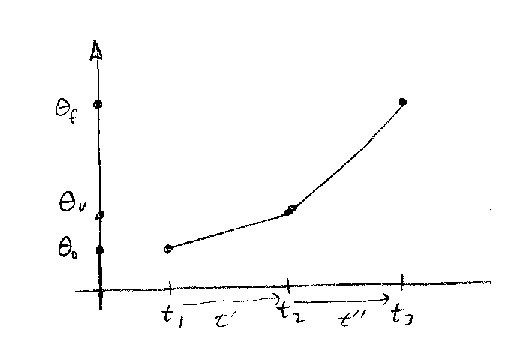
\includegraphics[width= 7.0cm]{figs07/00515.eps}
\caption{Two trajectories which join at a Via point ($\theta_V$).  Note that at this point we DO NOT have a smooth combined trajectory.}\label{twotrajectories}
\end{figure}



Let's introduce intermediate time variables so that we can keep each polynomial simple:

\[
t' = t - t_1       \qquad      t'' = t - t_2
\]

Then the two segments have the equations:

\[
\theta_1(t) = a_{10} + a_{11}t' + a_{12}t'^2 + a_{13}t'^3
\]
\[
\theta_2(t) = a_{20} + a_{21}t'' + a_{22}t''^2 + a_{23}t''^3
\]

There are thus 8 unknowns and we need eight equations to solve them:

\begin{enumerate}
  \item $\theta_0 = a_{10}$
  \item $\theta_f = a_{20} + a_{21}(t_{f2})+ a_{22}t_{f2}^2+a_{23}t_{f2}^3$
  \item $\theta_V = a_{20}$
  \item $\theta_V = a_{10}+a_{11}t_2 + a_{12}t_2^2+a_{13}t_2^3$
  \item $\dot{\theta}_1(t_1) = 0$
  \item $\dot{\theta}_2(t_3) = 0 = a_{21}+2a_{22}t_{f2}+3a_{23}t_{f2}^2$
  \item continuous velocity:
  \[
  \dot{\theta}_1(t_2) = \dot{\theta}_2{t_2} \to a_{11} + 2a_{12}t'_2+3a_{13}(t'_2)^2 = a_{21}
  \]
  \item continuous acceleration:
  \[
   \ddot{\theta}_1(t_2) = \ddot{\theta}_2{t_2} \to 2a_{12} + 6a_{13}t'_2 = 2 a_{22}
  \]
\end{enumerate}

where $t_{f2} = t_3-t_2$.    This can be solved readily and coded into a subroutine.

Such a trajectory might look like Figure \ref{continuousacceleration}.


\begin{figure}\centering
\includegraphics[width= 8.5cm]{figs07/00516.eps}
\caption{Two trajectories through a via point which are constrained to have continuous acceleration through the via point.}\label{continuousacceleration}
\end{figure}




The methods above could generate the trajectory for  a single joint, $\theta_i(t)$.   To move a robot arm from one pose to another, we work out the joint angles for the starting and ending poses (using inverse kinematics) and then plan a trajectory for each joint from its value in pose $A$ to its value in pose $B$ where each joint uses the same $t_f$.  This produces nicely synchronized and smooth motion.


\section{Cartesian Straight Line Motion}

\subsection{Position}
Sometimes it is not enough to plan the trajectory in the manipulator's joint space.   While the joint space trajectory may be smooth and attainable, we do not know where it goes between the start and end points in Cartesian space.  In the welding task shown below,  we need to make sure that the end effector motion goes in a straight line at a constant speed (Figure \ref{straightweld}).


\begin{figure}\centering
\includegraphics[width= 7.0cm]{figs07/00517.eps}
\caption{Cartesian straight line trajectory example: move the robot end effector so as to make a weld along a straight line joining two metal plates.}\label{straightweld}
\end{figure}



First, consider only the Cartesian end effector position and neglect orientation.  If we have $3\times1$ start position $P_A$ and end position $P_B$, we can generate a straight line path by linear interpolation.  Letting the time variable, $t$ be referenced to the start of the trajectory,

\[
P(t) = P_A + \frac{t}{t_f}(P_B-P_A)
\]

Then, at each sample of time, we can compute the joint positions with inverse kinematics. Note that for now we have neglected the starting and stopping accelerations.

Now, we know where the end effector is at each point along the Cartesian trajectory.  This is very important when obstacles might be present or when the trajectory is important to the task itself such as welding.  Two important issues however which must be considered with this method are choosing correctly between multiple solutions of the inverse kinematics, and dealing with trajectories which go through singular point (Figure \ref{trajectorymapping}).


\begin{figure}\centering
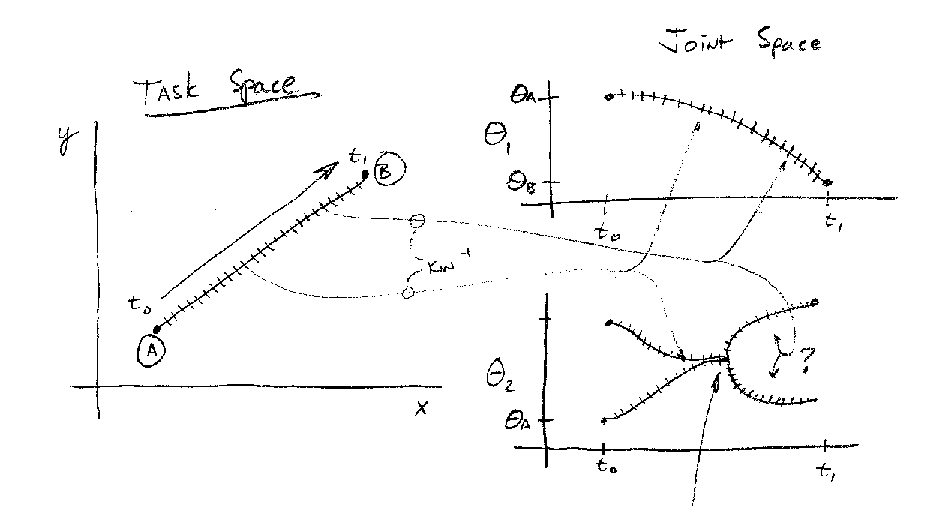
\includegraphics[width=14cm]{figs07/00518.eps}
\caption{An apparently simple trajectory in task space (left) can map to multiple and complex trajectories in joint space throught the inverse kinematics computation.}\label{trajectorymapping}
\end{figure}



On the left, a straight line trajectory is shown in the Cartesian end effector space of the robot.   The path is divided into sample points corresponding the linear interpolation function at several points in time.  On the right are the corresponding inverse kinematics solutions for two joints of the robot.   For $\theta_1$ (top) the inverse kinematics equations produce a single solution at each point for an unambiguous path.  However for $\theta_2$, the inverse kinematic equations produce two solutions.  Furthermore, at a singular point (see Chapter 5), the two solutions merge into one and afterwards diverge into two separate solutions again.  When controlling an actual robot, it is important that the algorithms consistently pick solutions which are close to each other in the joint space and make an intelligent choice of solutions when coming out of the singularity.  If control algorithms rely on the Jacobinan matrix inverse, they must be robust to the numerical problems which arise both at and in the
neighborhood of the singularity.

Not all paths will go through singular points, but trajectory generation algorithms which rely on inverse kinematics must be prepared to encounter them.

\subsection{Orientation}
What if the start and end points have different orientations of the end effector?  How do we interpolate orientation?   A naive approach might be to interpolate the orientation matrices from $R_A$ to $R_B$.   However it is easily shown that the interpolated matrices produced are not valid rotation matrices.  The answer is to convert the rotation matrices to one of the parameterized forms such as equivalent angle-axis form.   First, derive a rotation matrix which maps from the initial to final orientation.   Using the transform graph in Figure \ref{orientationtrajectory}, we can solve for $^A_BR$ as

\[
^A_BR = {^0_AR}^{-1}{^0_BR}
\]

\begin{figure}\centering
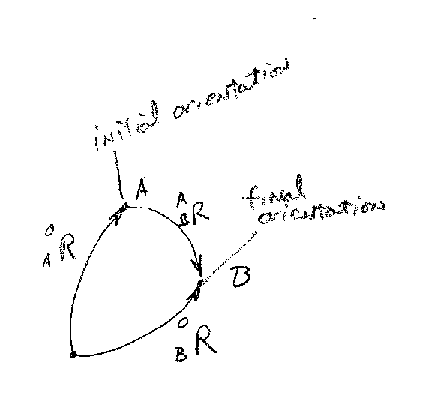
\includegraphics[width=6cm]{figs07/00519.eps}
\caption{To design a trajectory in orientation, we must find a way to interpolate ${^A_BR}$ but interpolation between two rotation matrices is not valid (see text).}\label{orientationtrajectory}
\end{figure}



where ${^0_AR}$ is the orientation at the initial point $A$ etc.   Using Chapter 2, we can convert $^A_BR$ to a fixed axis, $K$, and a rotation angle around that axis, $\theta_{AB}$.  Now we can keep $K$ fixed, and use one of the preceding trajectory generation methods for the angle $\theta_{AB}(t)$:

\[
\theta_{AB}(t) = \left (  S(t)   \right ) {\theta_{AB}}
\]
where, for the case of a third order trajectory,

\[
0 < S(t) < 1.0 \qquad 0 < t < t_{f} \qquad S(t) = a_1t + a_2t^2 + a_3t^3
\]

the first term, $a_0$ is zero because $^A_BR$ was defined relative to position $A$.
Then, the current rotation change is reconstructed from $K$ and $\theta_{AB}(t)$ and combined with $^0_AR$ to get the current rotation matrix
\[
^A_BR = {^0_AR}\, {^A_BR}(t)
\]

A similar method can be used with quaternions.






\subsection{Parameterized Cartesian Trajectories}

In the previous treatment of linear interpolated trajectories through cartesian space, we have ignored the infinite acceleration at the start.  Full consideration of this problem requires consideration of dynamics in future chapters, but we can at least address the concern by doing the linear interpolation with a parameter, $0 \leq p \leq  1$, and generating a smooth time function for $p$.  Considering position, we can convert our interpolation function to $p$ by


\[
P(t) = P_A + p(t)(P_B-P_A)
\]

where, for example,

\[
p(t) = a_0 + a_1t + a_2 t^2 + a_3 t^3
\]

We solve for $a_0$ to $a_3$ as in Section \ref{3rdPoly} where
\[
p(0) = 0   \qquad  p(t_f) = 1
\]
\[
\dot{p}(0) = \dot{p}(t_f) = 0
\]
giving
\[
a_0 = 0 \qquad a_1 = 0 \qquad a_2 = \frac{3}{t_f^2} \qquad a_3 = \frac{-2}{t_f^3}
\]

While this gives us a smoother straight line trajectory, we do not know which trajectories are attainable.   Also, a task like welding may require constant velocity over the entire path.  To properly perform the weld then we should use the linear-parabolic function instead of the polynomial for $p(t)$ and extend the length of the trajectory to  allow space for the manipulator to accelerate and decelerate before and after the weld line.




\section{Summary of Notation}

% Summary of Notation for Chapter  07

